\documentclass[ignorenonframetext,]{beamer}
\usepackage{amssymb,amsmath}
\usepackage{ifxetex,ifluatex}
\usepackage{fixltx2e} % provides \textsubscript
\ifxetex
  \usepackage{fontspec,xltxtra,xunicode}
  \defaultfontfeatures{Mapping=tex-text,Scale=MatchLowercase}
\else
  \ifluatex
    \usepackage{fontspec}
    \defaultfontfeatures{Mapping=tex-text,Scale=MatchLowercase}
  \else
    \usepackage[utf8]{inputenc}
  \fi
\fi
\usepackage{graphicx}
% Comment these out if you don't want a slide with just the
% part/section/subsection/subsubsection title:
\AtBeginPart{\frame{\partpage}}
\AtBeginSection{\frame{\sectionpage}}
\AtBeginSubsection{\frame{\subsectionpage}}
\AtBeginSubsubsection{\frame{\subsubsectionpage}}
\setlength{\parindent}{0pt}
\setlength{\parskip}{6pt plus 2pt minus 1pt}
\setlength{\emergencystretch}{3em}  % prevent overfull lines
\setcounter{secnumdepth}{0}


\begin{document}

\begin{frame}\frametitle{\texttt{fork}-ing, \texttt{merge}-ing and
\texttt{branch}-ing in \texttt{git}}

David L. Miller (University of Rhode Island)

St Andrews R user group talk

20 December 2012

\end{frame}

\begin{frame}[fragile]\frametitle{outline}

\begin{itemize}[<+->]
\item
  \texttt{git} re-cap
\item
  branches (and how to think about them)
\item
  merging
\item
  deleting branches
\item
  \texttt{stash}ing
\end{itemize}

\end{frame}

\begin{frame}[fragile]\frametitle{why \texttt{git}?}

\begin{itemize}[<+->]
\item
  \texttt{git} is the Delorean from \emph{Back to the Future}
\item
  time travel is possible (no roads required)
\item
  \texttt{\textless{}\textless{}extended metaphor\textgreater{}\textgreater{}}
  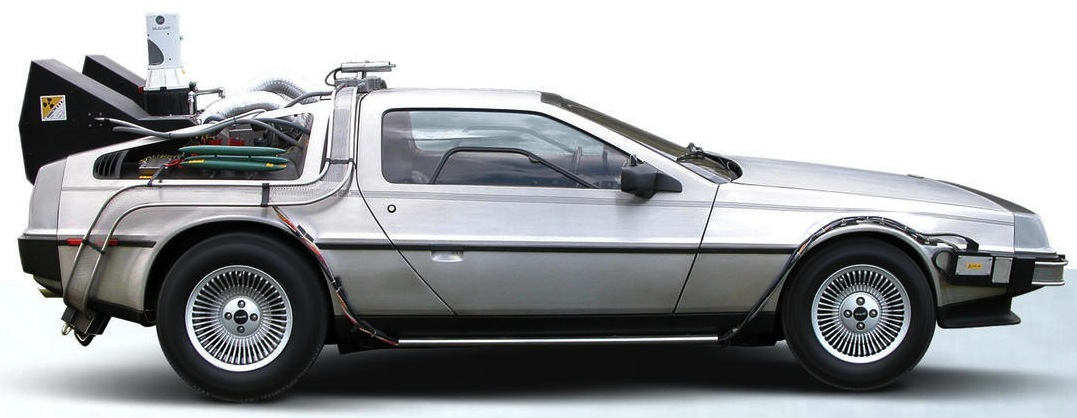
\includegraphics{delorean.jpg}
\end{itemize}

\end{frame}

\begin{frame}[fragile]\frametitle{re-cap}

let's start with a fresh \texttt{git} repo

\begin{verbatim}
$ mkdir ex
$ cd ex
$ git init
$ touch README
$ git add README
$ git commit -a -m "frivolous commit"
\end{verbatim}

\end{frame}

\begin{frame}\frametitle{why branches?}

\begin{itemize}[<+->]
\item
  contexts!
\item
  want to test some code but not screw other things up?
\item
  save results from different parameters
\end{itemize}

\end{frame}

\begin{frame}[fragile]\frametitle{branch example (1)}

Let's make a file called \texttt{row.max.R}:

\begin{verbatim}
# find the maximum in each row of a matrix -- slowly
row.max <- function(x){

  result <- c()

  for(i in 1:nrow(x)){
    this.max <- max(x[i,])
    result <- c(result, this.max)
  }
  return(result)
}
\end{verbatim}

\end{frame}

\begin{frame}[fragile]\frametitle{branch example (2)}

This does what you expect

\begin{verbatim}
> source("row.max.R")
> row.max(matrix(1:9,3,3))
[1] 7 8 9
\end{verbatim}

Yay! It works!

\begin{verbatim}
$ git add row.max.R
$ git commit -a -m "Brian Ripley would be proud"
\end{verbatim}

\end{frame}

\begin{frame}[fragile]\frametitle{branch example (3)}

\begin{itemize}[<+->]
\item
  But wait, I heard about this thing called \texttt{apply()}\ldots{}
\item
  What if that's better?
\item
  How do I try that out without angering other people on my project?
\item
  \texttt{branch}!
\end{itemize}

\end{frame}

\begin{frame}[fragile]\frametitle{branch example (4)}

First make a new branch and switch to it:

\begin{verbatim}
$ git branch apply
$ git checkout apply
Switched to branch 'apply'
\end{verbatim}

You can check which branch we're on using:

\begin{verbatim}
$ git branch
* apply
  master
\end{verbatim}

\end{frame}

\begin{frame}[fragile]\frametitle{branch example (5)}

Change the code:

\begin{verbatim}
# find the maximum in each row of a matrix
row.max <- function(x){
  return(apply(x,1,max))
}
\end{verbatim}

Try it:

\begin{verbatim}
> source("row.max.R")
> row.max(matrix(1:9,3,3))
[1] 7 8 9
\end{verbatim}

Hurrah!

\end{frame}

\begin{frame}[fragile]\frametitle{branch example (5)}

Now, we can commit our changes to this branch

\begin{verbatim}
$ git commit -a -m "now we use apply(), this is much better"
\end{verbatim}

we can switch back and forth between the branches and check where we
are:

\begin{verbatim}
$ git checkout master
$ git branch
* master
  apply
$ git checkout apply
$ git branch
  master
* apply
\end{verbatim}

\end{frame}

\begin{frame}\frametitle{branching - when is it useful?}

\begin{itemize}[<+->]
\item
  multiple sim results
\item
  want to check different parameter values
\item
  need to be careful with results if you want to access them all at once
\end{itemize}

\end{frame}

\begin{frame}[fragile]\frametitle{I started this, but I hate it}

nuke everything that's not committed

\begin{verbatim}
$ git reset --hard HEAD
\end{verbatim}

(this works anytime, but be careful!)

\end{frame}

\begin{frame}[fragile]\frametitle{merging -- very easy}

say we prefer \texttt{apply}, how do we make that our new
\texttt{master}?

\begin{verbatim}
$ git checkout apply
$ git merge --strategy=ours master
$ git checkout master
$ git merge apply
\end{verbatim}

\end{frame}

\begin{frame}[fragile]\frametitle{merging -- easy}

if changes are disjoint we \emph{fast-forward}

\begin{verbatim}
$ git commit -a -m "some changes"
$ git checkout master
$ git merge apply
\end{verbatim}

\end{frame}

\begin{frame}\frametitle{merging -- hard}

what if there were other changes?

\end{frame}

\begin{frame}[fragile]\frametitle{deleting branches}

To remove a local branch from your machine:

\begin{verbatim}
git branch -d the_local_branch
\end{verbatim}

\end{frame}

\begin{frame}[fragile]\frametitle{remember: all changes are local}

push your new branch back to github

\begin{verbatim}
$ git push origin apply
\end{verbatim}

remove a remote branch:

\begin{verbatim}
git push origin :the_remote_branch
\end{verbatim}

\end{frame}

\begin{frame}\frametitle{forking}

\begin{itemize}[<+->]
\item
  instead of branching, if you don't have write access
\item
  ``fork it''
\item
  copies repo to your github repos
\item
  then use a ``pull request'' to merge
\item
  all handled by github
\end{itemize}

\end{frame}

\begin{frame}[fragile]\frametitle{\texttt{git stash} for quick storage}

\begin{itemize}[<+->]
\item
  say you're working
\item
  need to do something else but don't want to commit
\item
  \texttt{stash} then come back to it
\item
  \texttt{HEAD} goes back to the last commit
\end{itemize}

\end{frame}

\begin{frame}[fragile]\frametitle{\texttt{stash} example}

\begin{verbatim}
$ git stash save "work in progress"
# work on something else
$ git commit -a -m "fixed!"
$ git stash pop
# back to where we were
\end{verbatim}

\end{frame}

\begin{frame}\frametitle{end}

\end{frame}

\end{document}
